\documentclass{article}
\usepackage[ruled,linesnumbered]{algorithm2e}
\usepackage{algpseudocode}
\usepackage{amsmath}
\usepackage{amssymb}
\usepackage{amsthm}
\usepackage{graphicx}
\usepackage{subfigure}
\usepackage{float}
\usepackage{amsfonts }
\usepackage{pdfpages}
\usepackage{epsfig}
\usepackage{graphicx}
\usepackage{arydshln}
\usepackage{verbatim}
\usepackage{subfigure}
\usepackage{enumerate}
\usepackage{rotating}
\usepackage{threeparttable}
\usepackage{caption}
\usepackage{epsfig}
\usepackage{cite}
\usepackage{times}
\usepackage{geometry}
\usepackage{setspace}
\usepackage[most]{tcolorbox}
\usepackage{tikz}

\definecolor{codegreen}{rgb}{0,0.6,0}
\definecolor{codegray}{rgb}{0.5,0.5,0.5}
\definecolor{codepurple}{rgb}{0.58,0,0.82}
\definecolor{backcolour}{rgb}{0.95,0.95,0.92}

\lstdefinestyle{SQL}{
    backgroundcolor=\color{backcolour},   
    commentstyle=\color{codegreen},
    keywordstyle=\color{magenta},
    numberstyle=\tiny\color{codegray},
    stringstyle=\color{codepurple},
    basicstyle=\footnotesize,
    breakatwhitespace=false,         
    breaklines=true,                 
    captionpos=b,                    
    keepspaces=true,                 
    numbers=left,                    
    numbersep=5pt,                  
    showspaces=false,                
    showstringspaces=false,
    showtabs=false,                  
    tabsize=2
}

\lstset{style=SQL}

\usetikzlibrary{positioning}
\usetikzlibrary{trees}
\geometry{a4paper}
\setstretch{1.2}
\usepackage[colorlinks,linkcolor=blue]{hyperref}
\begin{document}
\title{AI3613 Database System Concepts Homework 4}
\author{Kailing Wang 521030910356}
\date{May 21.2024}
\maketitle

\section*{Problem 1}

\begin{enumerate}[1.]
	\item A
	
	$500, 000/200 = 2500$ runs in the first pass, and $\lceil 2500/199 \rceil = 13$ runs in the second pass, and $\lceil 13/199 \rceil = 1$ is the final sorted file that we do not count. So the total number of runs is $2500+13=2513$.

	\item C

	Pass 0 for pre sort, pass 1 to merge and pass 2 to get the final sorted file. So the total number of passes is 3.

	\item C

	After pass 0, there are 2500 sorted blocks with 200 pages each. After pass 1, there are 13 sorted blocks, 12 of them should have $199\cdot 200$ pages and the rest one have rest of the pages.

	\item B

	In each pass, we read all and write all. So the total number of I/Os is $500, 000 \cdot 6 = 3, 000, 000$.
\end{enumerate}

\section*{Problem 2}
\begin{enumerate}
	\item a. D
	
	For partion, we need read in and out for all.

	b. B

	Need to read all partions once but output is ignored.

	\item C
	
	$P(R) + P(R) * P(S)=1081800$, $P(R) = 1800, P(S) = 600$. No way. We are to use 35 buffer pages to store outer table. $P(R) + P(R) * \lceil P(S)/(B-1)\rceil=33000$

	\item C

	Switch R and S. The result is the same by coincidence.

	\item a. C

	Only a sequential scan.

	b. A

	Suppose a==0, we need to join every tuple: the same cost as nested loop join.
\end{enumerate}

\section*{Problem 3}
\begin{center}
	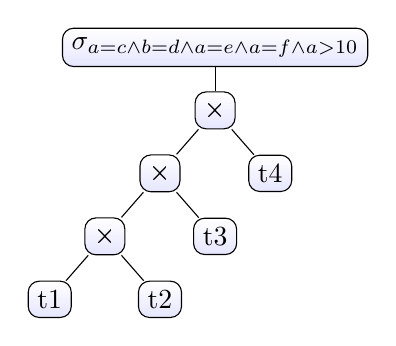
\begin{tikzpicture}[
	  every node/.style = {shape=rectangle, rounded corners, draw, align=center, top color=white, bottom color=blue!10},
	  level 1/.style={sibling distance=50mm, level distance=20mm},
	  level 2/.style={sibling distance=35mm, level distance=20mm},
	  level 3/.style={sibling distance=35mm, level distance=20mm},
	  edge from parent/.style={draw},
	  scale=0.4
	]
  
	  \node {$\sigma_{a=c \land b=d \land a=e \land a=f \land a>10}$}
	  child {node {×}
		child {node {×}
		  child {node {×}
			child {node {t1}}
			child {node {t2}}
		  }
		  child {node {t3}}
		}
		child {node {t4}}
	  };
	\end{tikzpicture}
  \end{center}

\[
\sigma_{a=c \land b=d \land a=e \land a=f \land a>10} \left( t1 \times t2 \times t3 \times t4 \right),
\]

\[
\sigma_{a>10}(\sigma_{a=c \land b=d}(\sigma_{a=e}(\sigma_{a=f}(t1 \times t2 \times t3 \times t4))))
\]

Use theta join to replace cross join:
\[
(\sigma_{a>10}(t1) \Join_{a=c\land b=d} t2) \Join_{a=e} t3 \Join_{a=f} t4
\]

\begin{center}
	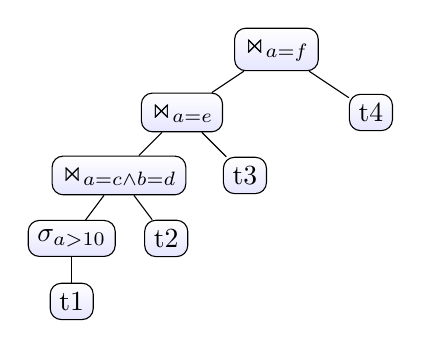
\begin{tikzpicture}[
	  every node/.style = {shape=rectangle, rounded corners, draw, align=center, top color=white, bottom color=blue!10},
	  level 1/.style={sibling distance=60mm, level distance=20mm},
	  level 2/.style={sibling distance=40mm, level distance=20mm},
	  level 3/.style={sibling distance=30mm, level distance=20mm},
	  edge from parent/.style={draw},
	  scale=0.4
	]
  
	  \node {$\Join_{a=f}$}
	  child {node {$\Join_{a=e}$}
		child {node {$\Join_{a=c \land b=d}$}
		  child {
			node {$\sigma_{a>10}$}
			child {node {t1}}
			}
		  child {node {t2}}
		}
		child {node {t3}}
	  }
	  child {node {t4}};
	\end{tikzpicture}
\end{center}

\section*{Problem 4}
\begin{enumerate}[1.]
	\item The query can be formulated as
	
	$\Pi_{course\_id} \left( \sigma_{semester = 'Fall' \land year = 2023}(S) \ltimes_{S.course\_id = T.course\_id} \sigma_{semester = 'Spring' \land year = 2024} (\rho_{T}(S)) \right)$
	
	The query plan is as follows:
	\begin{center}
		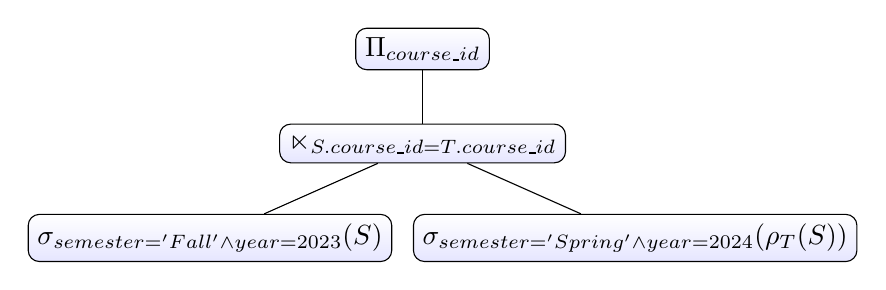
\begin{tikzpicture}[
		  every node/.style = {shape=rectangle, rounded corners, draw, align=center, top color=white, bottom color=blue!10},
		  level 1/.style={sibling distance=60mm, level distance=20mm},
		  level 2/.style={sibling distance=90mm, level distance=20mm},
		  level 3/.style={sibling distance=150mm, level distance=20mm},
		  edge from parent/.style={draw},
		  scale=0.6
		]
	  
		  \node {$\Pi_{course\_id}$}
		  child {node {$\ltimes_{S.course\_id = T.course\_id}$}
			child {node {$\sigma_{semester = 'Fall' \land year = 2023} (S)$}}
			child {node {$\sigma_{semester = 'Spring' \land year = 2024} (\rho_{T}(S))$}}
		  };
		\end{tikzpicture}
	  \end{center}
	
	\item Similar to the given query, antijoin indicates not exists. The query
	
	\[ 
	\Pi_{\text{gpa}}(\text{Students} \overline{\ltimes}_{\text{Students.stu\_id} = \text{Punished.punished\_stu\_id}} (\text{Punished}))
	\]

	\begin{lstlisting}
	SELECT S.gpa
	FROM Students as S
	WHERE S.stu_id NOT IN (
		SELECT P.punished_stu_id
		FROM Punishment as P
	);\end{lstlisting}
	
	\item

	\begin{algorithm}[H]
	\DontPrintSemicolon
	\SetAlgoNoEnd
	\SetAlgoNoLine

	\SetKwInput{KwData}{Input}
	\SetKwInput{KwResult}{Output}
	
	% \KwData{$R$, $S$ two relations, $\overline{\ltimes}$ a predicate}
	% \KwResult{Result of $R \bowtie_{\theta} S$}
	
	\For{each page $P_r$ in $R$}{
		\For{each page $P_s$ in $S$}{
			\For{each tuple $t_r$ in $P_r$}{
				\For{each tuple $t_s$ in $P_s$}{
					\If{$\theta(t_r, t_s)$}{
						break\;
					}
					add $t_r \bowtie t_s$ to the result\;
				}
			}
		}
	}
	
	\caption{$R \overline{\ltimes}_{\theta} S$}
	\end{algorithm}
	
\end{enumerate}

\section*{Problem 5}
\begin{tcolorbox}[colback=gray!10, breakable]
	How long does it take you to finish the assignment? Give a score (1,2,3,4,5) to the difficulty of each problem. List all your collaborators if you have any.
\end{tcolorbox}
Abut 3 hours including review. 2, 2, 3, 3.
\end{document}